%% -*- coding: utf-8 -*-
\documentclass[12pt,a4paper]{scrartcl} 
\usepackage[utf8]{inputenc}
\usepackage[english,russian]{babel}
\usepackage{indentfirst}
\usepackage{misccorr}
\usepackage{graphicx}
\usepackage{amsmath}
\usepackage[left=25mm, top=20mm, right=20mm, bottom=20mm, nohead, nofoot]{geometry}
\begin{document}
  \begin{titlepage}
    \begin{center}
      \large
      МИНИСТЕРСТВО НАУКИ И ВЫСШЕГО ОБРАЗОВАНИЯ РОССИЙСКОЙ ФЕДЕРАЦИИ
      
      Федеральное государственное бюджетное образовательное учреждение высшего образования
      
      \textbf{АДЫГЕЙСКИЙ ГОСУДАРСТВЕННЫЙ УНИВЕРСИТЕТ}
      \vspace{0.25cm}
      
      Инженерно-физический факультет
      
      Кафедра автоматизированных систем обработки информации и управления
      \vfill

      \vfill
      
      \textsc{Отчет по практике}\\[5mm]
      
      {\LARGE Решение системы линейных алгебраических уравнений методом Гаусса-Жордана.}
      \bigskip
      
      1 курс, группа 1ИВТ
    \end{center}
    \vfill
    
    \newlength{\ML}
    \settowidth{\ML}{«\underline{\hspace{0.7cm}}» \underline{\hspace{2cm}}}
    \hfill\begin{minipage}{0.5\textwidth}
      Выполнил:\\
      \underline{\hspace{\ML}} Д.\,Э.~Небольсин\\
      «\underline{\hspace{0.7cm}}» \underline{\hspace{2cm}} 2023 г.
    \end{minipage}%
    \bigskip
    
    \hfill\begin{minipage}{0.5\textwidth}
      Руководитель:\\
      \underline{\hspace{\ML}} С.\,В.~Теплоухов\\
      «\underline{\hspace{0.7cm}}» \underline{\hspace{2cm}} 2023 г.
    \end{minipage}%
    \vfill
    
    \begin{center}
      Майкоп, 2023 г.
    \end{center}
  \end{titlepage}
\label{sec:intro}


\large\tableofcontents

\newpage

\section{Теория}
\subsection{Техническое задание}
\textbf {Задание:}

Решение системы линейных алгебраических уравнений методом Гаусса-Жордана.

\subsection{Теоретическая часть}

Метод Гаусса - Жордана (метод полного исключения неизвестных) - метод, который используется для решения квадратных систем линейных алгебраических уравнений, нахождения обратной матрицы, нахождения координат вектора в заданном базисе или отыскания ранга матрицы. Метод является модификацией метода Гаусса. 

Алгоритм:\textit{}

1)	Выбирают первый слева столбец матрицы, в котором есть хоть одно отличное от нуля значение.\textit{}

2)	Если самое верхнее число в этом столбце ноль, то меняют всю первую строку матрицы с другой строкой матрицы, где в этой колонке нет нуля.\textit{}

3)	Все элементы первой строки делят на верхний элемент выбранного столбца.\textit{}

4)	Из оставшихся строк вычитают первую строку, умноженную на первый элемент соответствующей строки, с целью получить первым элементом каждой строки (кроме первой) ноль.\textit{}

5)	Далее проводят такую же процедуру с матрицей, получающейся из исходной матрицы после вычёркивания первой строки и первого столбца.\textit{}

6)	После повторения этой процедуры n-1 раз получают верхнюю треугольную матрицу.\textit{}

7)	Вычитают из предпоследней строки последнюю строку, умноженную на соответствующий коэффициент, с тем, чтобы в предпоследней строке осталась только 1 на главной диагонали.\textit{}

8)	Повторяют предыдущий шаг для последующих строк. В итоге получают единичную матрицу и решение на месте свободного вектора (с ним необходимо проводить все те же преобразования).

\newpage

\section{Ход работы}
\label{sec:exp}

\subsection{Код приложения}
\label{sec:exp:code}
\begin{verbatim}
#include <iostream>
#include <conio.h>
#include <stdio.h>
#include <string>
#include <cmath>

using namespace std;

double getValue(int s, int c, int n, double *m)
{
    return m[s * (n + 1) + c];
}

void setValue(double v, int s, int c, int n, double *m)
{
    m[s * (n + 1) + c] = v;
}

void printMatrix(int n, double *m)
{
    for (int s = 0; s < n; s++)
    {
        for (int c = 0; c < n + 1; c++)
        {
            cout << getValue(s, c, n, &m[0]) << "  ";
        }
        cout << "\n";
    }
    cout << "\n";
}

void setLine(int s, int n, double *m)
{
    double tmp;

    for (int i = 0; i < n; i++)
    {
        if (getValue(i, s, n, m) != 0)
        {
            if (i != 0)
            {
                for (int j = s; j < n + 1; j++)
                {
                    tmp = getValue(s, j, n, m);
                    setValue(getValue(i, j, n, m), s, j, n, m);
                    setValue(tmp, i, j, n, m);
                }
            }
            break;
        }
    }
}

void makeLine(int s, int n, double *m)
{
    double k = getValue(s, s, n, m);
    for (int i = s; i < n + 1; i++)
    {
        setValue(getValue(s, i, n, m) / k, s, i, n, m);
    }
}

void setZeroLeftBottom(int s, int n, double *m)
{
    double tmp, tmp1, k;
    for (int i = s + 1; i < n; i++)
    {
        k = getValue(i, s, n, m);
        for (int j = s; j < n + 1; j++)
        {
            tmp = getValue(s, j, n, m);
            tmp1 = getValue(i, j, n, m);
            setValue(tmp * (-k) + tmp1, i, j, n, m);
        }
    }
}

void setZeroRightTop(int s, int n, double *m)
{
    double tmp, tmp1, k;
    for (int i = s - 1; i >= 0; i--)
    {
        k = getValue(i, s, n, m);
        for (int j = s; j < n + 1; j++)
        {
            tmp = getValue(s, j, n, m);
            tmp1 = getValue(i, j, n, m);
            setValue(tmp * (-k) + tmp1, i, j, n, m);
        }
    }
}

bool isNull (float value)
{
    if (std::abs(value) < 0.0000001)
    {
        return true;
    }
    return false;
}

int main(void)
{
    int n, s, c;

    cout << "Размерность = ";
    cin >> n;

    double matrix[n][n + 1];

    for (s = 0; s < n; s++)
    {
        cout << "\n";
        for (c = 0; c < n + 1; c++)
        {
            cout << "a[" << s << "][" << c << "] = ";
            cin >> matrix[s][c];
        }
    }
    cout << "\n";
    printMatrix(n, &matrix[0][0]);

    cout << "Левый угол\n";

    for (int s = 0; s < n; s++)
    {
        setLine(s, n, &matrix[0][0]);

        if (isNull(getValue(s, s, n, &matrix[0][0])))
        {
            if (isNull(getValue(s, n, n, &matrix[0][0])))
            {
                cout << "Бесконечное количество решений";
            }
            else
            {
                cout << "Решений нет";
            }
            return 0;
        }

        makeLine(s, n, &matrix[0][0]);

        setZeroLeftBottom(s, n, &matrix[0][0]);

        printMatrix(n, &matrix[0][0]);
    }

    cout << "Правый угол\n";

    for (int s = n - 1; s >= 0; s--)
    {
        setZeroRightTop(s, n, &matrix[0][0]);
        printMatrix(n, &matrix[0][0]);
    }

    cout << "Решение уравнения\n";
    for (int i = 0; i < n; i++)
    {
        cout    << "X["<< i+1 << "] = " 
                << getValue(i, n, n, &matrix[0][0]) 
                << "\n";
    }
}
\end{verbatim}

\subsection{Работа программы}
\subsubsection{Пример системы уравнений с решением}



\begin{wrapfigure}
  \begin{center}
    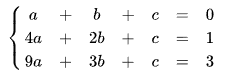
\includegraphics[width=0.3\textwidth]{estresh.png}
  \end{center}
  \caption{Рис.1  Пример системы линейных алгебраических уравнений}\label{fig:ex}
\end{wrapfigure}

\begin{wrapfigure}
  \begin{center}
    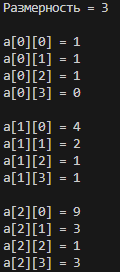
\includegraphics[width=0.25\textwidth]{vhoddan1.png}
  \end{center}
  \caption{Рис.2  Пример входных данных}\label{fig:ex}
\end{wrapfigure}

\begin{wrapfigure}
  \begin{center}
    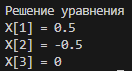
\includegraphics[width=0.25\textwidth]{imeetresh.png}
  \end{center}
  \caption{Рис.3  Пример вывода данных}\label{fig:ex}
\end{wrapfigure}

\newpage
\subsubsection{Пример системы уравнений без решения}

\begin{wrapfigure}
  \begin{center}
    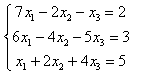
\includegraphics[width=0.3\textwidth]{netresh.png}
  \end{center}
  \caption{Рис.4  Пример системы линейных алгебраических уравнений}\label{fig:ex}
\end{wrapfigure}

\begin{wrapfigure}
  \begin{center}
    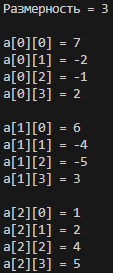
\includegraphics[width=0.25\textwidth]{vhoddan2.png}
  \end{center}
  \caption{Рис.5  Пример входных данных}\label{fig:ex}
\end{wrapfigure}

\begin{wrapfigure}
  \begin{center}
    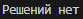
\includegraphics[width=0.2\textwidth]{neimeetresh.png}
  \end{center}
  \caption{Рис.6  Пример вывода данных}\label{fig:ex}
\end{wrapfigure}

\newpage
\subsubsection{Пример системы уравнений с бесконечным количеством решений}

\begin{wrapfigure}
  \begin{center}
    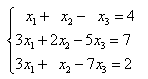
\includegraphics[width=0.3\textwidth]{infinity.png}
  \end{center}
  \caption{Рис.7  Пример системы линейных алгебраических уравнений}\label{fig:ex}
\end{wrapfigure}

\begin{wrapfigure}
  \begin{center}
    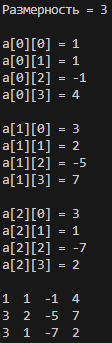
\includegraphics[width=0.25\textwidth]{vhoddan3.png}
  \end{center}
  \caption{Рис.8  Пример входных данных}\label{fig:ex}
\end{wrapfigure}

\begin{wrapfigure}
  \begin{center}
    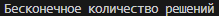
\includegraphics[width=0.5\textwidth]{infinityresh.png}
  \end{center}
  \caption{Рис.9  Пример вывода данных}\label{fig:ex}
\end{wrapfigure}

\end{document}
